\section{Method}
\label{sec:method}

\begin{figure}[t]
  \centering
  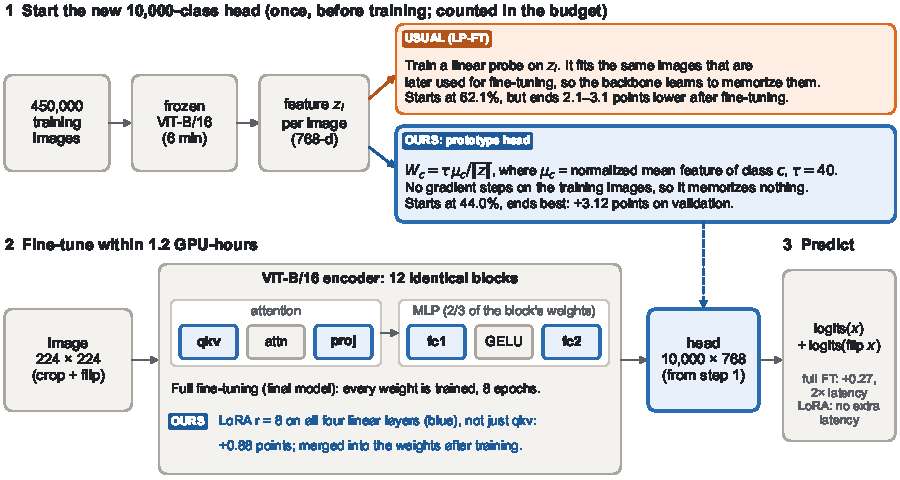
\includegraphics[width=\linewidth]{figures/fig_pipeline.pdf}
  \caption{\textbf{Our pipeline, with our changes in blue.}
  (1)~We start the new head from class prototypes of the frozen backbone, not from the usual LP-FT linear probe (orange), which is fitted on the same training images.
  (2)~We fine-tune all weights, or LoRA on all four linear layers (the reference: qkv only).
  (3)~Full fine-tuning adds the logits of each image and its mirror image. Gains are from \cref{sec:experiments}.}
  \label{fig:pipeline}
\end{figure}

\Cref{fig:pipeline} shows our pipeline.
Let $f_\theta$ map an image $x$ to its final \texttt{[CLS]} feature $z = f_\theta(x) \in \mathbb{R}^{768}$, and let $h(z) = Wz + b$ with $W \in \mathbb{R}^{10000 \times 768}$ be the new head.

\paragraph{What we changed, and why.}
We started from the recipes in the project description and changed five things, each after a test on the holdout (\cref{sec:process}):
\begin{enumerate}[leftmargin=*,itemsep=1pt,topsep=2pt]
  \item \textbf{A prototype head instead of a linear-probe head} (\cref{sec:head-init}). Our first runs used LP-FT. When LoRA's training loss went \emph{up} in its first epoch, we traced the problem to the probe, which had been fitted on the same images. A prototype head is not trained on them at all. This is our main change: $+$2.1 to $+$3.1 points.
  \item \textbf{LoRA on all four linear layers, not only qkv}, because the MLP holds two thirds of each block's weights: $+$0.88 points with 1.375\% of the backbone.
  \item \textbf{A different schedule for each final model}: 8 epochs for full fine-tuning, which keeps improving, and 3 for LoRA, which gets worse with more epochs (\cref{sec:ablation-lora}).
  \item \textbf{A budget clock that counts every GPU second}, including the feature extraction for the head, and shortens the schedule if a run would go over the budget (\cref{sec:budget}).
  \item \textbf{Flip test-time augmentation} for the full fine-tuning model: $+$0.27 points for twice the latency.
\end{enumerate}

\subsection{Backbone and budget}
\label{sec:budget}

\paragraph{Backbone.}
We use the timm \citep{wightman2019timm} checkpoint \nolinkurl{vit_base_patch16_224.augreg2_in21k_ft_in1k}, the backbone that the project description recommends: ViT-B/16 pretrained on ImageNet-21k with AugReg and fine-tuned on ImageNet-1k.
It has 85,798,656 parameters; its 1,000-class head is replaced by a new 10,000-class head (7,690,000 parameters).
We keep it in every experiment: after the deadline we checked two ImageNet-21k-only ViT-B/16 models that the project description also lists, and a linear probe on their frozen features is worse on our holdout (61.05\% and 51.07\% \vs 61.94\%).

\paragraph{Compute budget.}
The project allows 2\,h$\times$48\,GB $=$ 96\,GB$\cdot$h per training run ($\pm$10\%), which is 1.2 hours on our 80\,GB A100.
Our clock counts all GPU work for training (head initialization with feature extraction, all optimizer steps and the holdout check after every epoch), but not unpacking the data, saving checkpoints or the final predictions.
The code times training steps 20--120; if the planned epochs would use more than 97\% of the budget, it shortens the cosine schedule, and it stops training at 1.05$\times$ the budget.
Every run in our results finished within 1.06 GPU-hours; the only longer run is a post-deadline test that is not part of our results (\cref{sec:post}).

\subsection{Starting the 10,000-class head}
\label{sec:head-init}

The head is the largest new part of the model, and each of its rows is trained on at most 45 images.
A random head gives almost uniform logits (initial loss $\approx \ln 10000 = 9.2$), so early in training the backbone gets large, noisy gradients from it.
We compare three ways to start the head.

\paragraph{Random.} timm's default initialization of a new linear layer.

\paragraph{Prototype head (ours).}
With the frozen pretrained backbone, we extract the features $z_i$ of all training images once.
We then copy the L2-normalized class means into the head \citep{snell2017prototypical,qi2018imprinted}:
\begin{equation}
  \mu_c = \frac{\sum_{i:\,y_i=c} \hat z_i}{\big\|\sum_{i:\,y_i=c} \hat z_i\big\|}, \quad
  W_c = \frac{\tau}{\overline{\|z\|}}\, \mu_c, \quad b_c = 0,
  \label{eq:proto}
\end{equation}
where $\hat z_i = z_i / \|z_i\|$ and $\overline{\|z\|}$ is the mean feature norm, so each logit is about $\tau \cos(z, \mu_c)$.
We pick the temperature $\tau$ from $\{5, 10, 15, 20, 30, 40, 60, 80\}$ by the cross-entropy on 10,000 training features, which gives $\tau = 40$.
Without any training, this head already reaches 44.0\% holdout accuracy.
Feature extraction takes 6--7 minutes on an A100, and we count this time in every run's GPU-hours.
The head knows the class structure from the start, but it has never been fitted to single training images, so it has nothing to memorize.

\paragraph{Linear-probe (LP) head.}
Starting from the prototype head, we train $(W, b)$ on the cached frozen features for 10 epochs (AdamW, learning rate $10^{-3}$, weight decay $10^{-4}$, batch size 4,096, cosine decay, label smoothing 0.1).
This reaches 62.1\% holdout accuracy in a few seconds and is the first stage of LP-FT \citep{kumar2022lpft}.
It was our first design, chosen so that a random head would not distort the features.

\subsection{Adaptation methods}
\label{sec:peft}

\paragraph{Full fine-tuning.}
All backbone and head weights are trained with AdamW \citep{loshchilov2019adamw} at learning rate $10^{-4}$ and weight decay 0.05 (none on biases, normalization parameters, the class token and position embeddings).
We use layer-wise learning-rate decay of 0.75 \citep{bao2022beit}, drop path 0.1 \citep{huang2016stochastic}, a linear warmup (one epoch for runs of 6 or more epochs, 0.3 epochs for 3-epoch runs) and a cosine decay to zero \citep{loshchilov2017sgdr}.
Other settings are batch size 256, bf16 mixed precision, gradient clipping at norm 1 and label smoothing 0.1 \citep{szegedy2016rethinking}.
Training images get RandomResizedCrop (scale 0.25--1) and a horizontal flip; for evaluation, images are resized to 248 pixels and center-cropped to 224.
At test time, the final full fine-tuning model adds the logits of each image and of its horizontal flip \citep{krizhevsky2012imagenet}.

\paragraph{LoRA.}
For a frozen linear layer $W_0 \in \mathbb{R}^{d_\text{out} \times d_\text{in}}$, LoRA \citep{hu2022lora} computes
\begin{equation}
  y = W_0 x + \tfrac{\alpha}{r} B A x,
  \label{eq:lora}
\end{equation}
where $A \in \mathbb{R}^{r \times d_\text{in}}$ and $B \in \mathbb{R}^{d_\text{out} \times r}$ are trained and $B$ starts at zero, so training starts exactly from the pretrained model.
We use the PEFT library \citep{mangrulkar2022peft} with $r = 8$ and $\alpha = 16$.
timm joins the query, key and value projections into one \texttt{qkv} layer, so LoRA on \texttt{qkv} (294,912 parameters, 0.344\% of the backbone) adapts all three.
Our final LoRA model applies LoRA to all four linear layers of every block (\texttt{qkv}, \texttt{proj}, \texttt{fc1}, \texttt{fc2}), for 1,179,648 parameters (1.375\%).
The LoRA weights and the head use learning rate $10^{-3}$ and weight decay $10^{-4}$, with no LoRA dropout.
After training, $\tfrac{\alpha}{r}BA$ is added into $W_0$, so inference uses exactly the base model.

\paragraph{Other methods.}
AdaptFormer \citep{chen2022adaptformer} adds a bottleneck branch next to the MLP of each block,
\begin{equation}
  x_{l+1} = x' + \mathrm{MLP}(\mathrm{LN}(x')) + s \cdot W_\text{up}\,\mathrm{ReLU}(W_\text{down} x'),
  \label{eq:adaptformer}
\end{equation}
where $x'$ is the output of the attention sub-block; we use width 64, scale $s = 0.1$, dropout 0.1 and a zero-initialized $W_\text{up}$.
The serial Adapter \citep{houlsby2019adapter} applies the same bottleneck to the MLP output, before the residual addition and without a scale.
Both have 1,189,632 parameters (1.387\%) and cannot be merged into the backbone.
BitFit \citep{benzaken2022bitfit} trains only the bias vectors of all linear and normalization layers (102,912 parameters, 0.120\%).
Partial fine-tuning trains the last $K$ blocks and the final normalization layer; one block has 7,087,872 parameters (8.26\% of the backbone).
\Cref{tab:params} in the appendix shows how each count is computed.
In every run except zero-shot the head is also trained; since it alone has 7.69M parameters, we report trainable parameters without it, as in the project's 0.34\% LoRA reference.
